\documentclass[11pt,letterpaper]{article}

\usepackage[margin=1in]{geometry}
\usepackage{amsmath,amssymb,mathtools}
\usepackage{xcolor}
\usepackage[most]{tcolorbox}
\usepackage{fancyhdr}
\usepackage{titlesec}
\usepackage{tocloft}
\usepackage{enumitem}
\usepackage{hyperref}

\hypersetup{colorlinks=false, pdfborder={0 0 0}, pdftitle={Physics -- Lecture 1: Units, Measurement Systems, and Vectors}}

% ---------- Colors ----------
\definecolor{boxblue}{RGB}{31,74,121}
\definecolor{boxgreen}{RGB}{27,94,32}
\definecolor{boxpurple}{RGB}{106,27,154}
\definecolor{boxred}{RGB}{140,20,20}
\definecolor{boxorange}{RGB}{198,93,10}
\definecolor{boxteal}{RGB}{13,110,110}

% ---------- Section / subsection formatting ----------
\titleformat{\section}{\normalfont\Large\bfseries\color{boxblue}}{\thesection}{0.6em}{}
\titlespacing*{\section}{0pt}{1.3em}{0.9em}
\titleformat{\subsection}{\normalfont\large\bfseries\color{boxblue}}{\thesubsection}{0.6em}{}
\titlespacing*{\subsection}{0pt}{1.4em}{0.6em}

% ---------- Table of contents styling ----------
\renewcommand{\cftsecfont}{\bfseries\color{boxblue}}
\renewcommand{\cftsecpagefont}{\bfseries\color{boxblue}}
\renewcommand{\cftsubsecfont}{\color{boxblue}}
\renewcommand{\cftsubsecpagefont}{\color{boxblue}}
\renewcommand{\cftsecleader}{\cftdotfill{\cftsecdotsep}}
\renewcommand{\cftsecdotsep}{4.5}
\setlength{\cftbeforesecskip}{6pt}
\setlength{\cftbeforesubsecskip}{2pt}

% ---------- Header / footer ----------
\setlength{\headheight}{14pt}
\pagestyle{fancy}
\fancyhf{}
\fancyhead[L]{\textit{Physics Notes --- Lecture 1}}
\fancyhead[R]{\thepage}
\renewcommand{\headrulewidth}{0.5pt}
\fancyfoot[C]{Units, Measurement Systems \& Vectors}

\fancypagestyle{plain}{%
  \fancyhf{}
  \fancyfoot[C]{Units, Measurement Systems \& Vectors}
  \renewcommand{\headrulewidth}{0pt}
}

% ---------- Source-reference tag ----------
\newcommand{\srctag}[2]{\textcolor{gray}{\normalfont\itshape\footnotesize [ \textbf{m.}~#1, \textbf{c.}~#2 ]}}

% ---------- Box environments ----------
\newtcolorbox{introbox}[3]{
  breakable, colback=white, colframe=boxblue, coltitle=white, fonttitle=\bfseries,
  boxrule=1pt, arc=0.4mm, left=6pt, right=6pt, top=5pt, bottom=5pt,
  title={#1\hfill{\normalfont\itshape\footnotesize\color{white} m.~#2, c.~#3}}
}

\newtcolorbox{defbox}[1]{
  breakable, colback=white, colframe=boxgreen, coltitle=white, fonttitle=\bfseries,
  boxrule=1pt, arc=0.4mm, left=6pt, right=6pt, top=5pt, bottom=5pt,
  title={Definition: #1}
}

\newtcolorbox{rulebox}[1]{
  breakable, colback=white, colframe=boxblue, coltitle=white, fonttitle=\bfseries,
  boxrule=1pt, arc=0.4mm, left=6pt, right=6pt, top=5pt, bottom=5pt,
  title={Theorem / Rule: #1}
}

\newtcolorbox{derivbox}[1]{
  breakable, colback=white, colframe=boxpurple, coltitle=white, fonttitle=\bfseries,
  boxrule=1pt, arc=0.4mm, left=6pt, right=6pt, top=5pt, bottom=5pt,
  title={Derivation: #1}
}

\newtcolorbox{examplebox}[1]{
  breakable, colback=white, colframe=boxred, coltitle=white, fonttitle=\bfseries,
  boxrule=1pt, arc=0.4mm, left=6pt, right=6pt, top=5pt, bottom=5pt,
  title={Example: #1}
}

\newtcolorbox{plotbox}[2]{
  breakable, colback=white, colframe=boxteal, coltitle=white, fonttitle=\bfseries,
  boxrule=1pt, arc=0.4mm, left=6pt, right=6pt, top=5pt, bottom=5pt,
  title={Figure~#1\ \ ---\ \ #2}
}

\newtcolorbox{watchbox}{
  breakable, colback=white, colframe=boxorange, coltitle=white, fonttitle=\bfseries,
  boxrule=1pt, arc=0.4mm, left=6pt, right=6pt, top=5pt, bottom=5pt,
  title=Watch out
}

\newtcolorbox{topicsbox}{
  breakable, colback=white, colframe=boxblue, boxrule=1pt, arc=1mm,
  left=10pt, right=10pt, top=7pt, bottom=7pt
}

% ---------- Practice-problem group heading (not added to ToC) ----------
\newcommand{\probgroup}[3]{%
  \bigskip
  \noindent{\large\bfseries\color{boxblue} #1.\ #2\ \textcolor{gray}{\normalfont\itshape\footnotesize [ \textbf{m.}~#3 ]}}\par\smallskip
}

\setlist[enumerate,1]{leftmargin=1.6em}
\setlist[itemize,1]{leftmargin=1.6em}

\newcommand{\dd}[2]{\frac{\mathrm{d}#1}{\mathrm{d}#2}}

\usepackage{booktabs,longtable,array}
\setlength{\emergencystretch}{2em}

\usepackage{graphicx,tikz}
\usetikzlibrary{arrows.meta,calc}
\newcommand{\vect}[1]{\boldsymbol{#1}}
\newcommand{\uv}[1]{\hat{\boldsymbol{#1}}}
\newcommand{\unit}[1]{\,\mathrm{#1}}
\newcommand{\degree}{^{\circ}}
\newcommand{\bookref}[2]{\textcolor{gray}{\footnotesize Young--Freedman, Sec.~#1, pp.~#2.}}

\begin{document}
\hypersetup{pageanchor=false}
\begin{titlepage}
\thispagestyle{empty}
\begin{center}
\vspace*{0.8cm}
{\color{boxblue}\fontsize{24.88}{30}\selectfont Physics Notes}\\[0.4cm]
{\color{boxblue}\Large Lecture 1: Units, Measurement Systems,\\[0.12cm] and Vectors}\\[0.5cm]
{\large  Lecture Notes and Worked Examples}\\[0.6cm]
\begin{minipage}{0.86\textwidth}
\centering\itshape
These notes develop the material covered in our first lecture, following Young and Freedman, \emph{University Physics with Modern Physics}, 13th edition, Chapter 1, with the additional unit systems and exercises discussed in class.

\medskip
Green boxes give definitions, blue boxes collect rules, purple boxes explain derivations, red boxes contain worked examples, and orange boxes flag common mistakes. The supplied textbook Figures 1.27 and 1.29 are included and explained. Practice problems are collected at the end of the notes.
\end{minipage}
\end{center}
\vfill
\tableofcontents
\thispagestyle{empty}
\end{titlepage}
\hypersetup{pageanchor=true}

\section{Units, Measurement Systems, and Vectors}
\begin{topicsbox}

\medskip
\textbf{Notation.} Bold symbols such as $\vect A$ denote vectors. The corresponding plain symbol $A=|\vect A|$ denotes a nonnegative magnitude. Unless a question says otherwise, use a right-handed Cartesian coordinate system, measure planar direction angles counterclockwise from $+x$, and set the calculator to \textbf{degree mode} for angles written in degrees.
\end{topicsbox}

\subsection{Physical Quantities and Measurement}
\bookref{1.3--1.4}{4--7}

\begin{defbox}{A physical quantity needs a number and a unit}
A physical quantity is something that can be measured or calculated from measurements. Write it as
\[
 \boxed{\text{quantity}=\text{numerical value}\times\text{unit}.}
\]
For example, a length $\ell=1.25\unit{m}$ has numerical value $1.25$ when its unit is the metre. The \emph{same length} is $125\unit{cm}$: changing the unit changes the number, not the physical quantity.
\begin{center}
\begin{tabular}{lll}
\toprule
Quantity & Example from the lecture & Meaning of the unit\\
\midrule
Length & $2.5\unit{m}$ & metre\\
Mass & $12\unit{kg}$ & kilogram\\
Time interval & $3\unit{s}$ & second\\
Temperature & $300\unit{K}$ & kelvin\\
Force magnitude & $15\unit{N}$ & newton\\
Energy & $50\unit{J}$ & joule\\
Pressure & $100\unit{kPa}$ & kilopascal\\
\bottomrule
\end{tabular}
\end{center}
\end{defbox}

\begin{examplebox}{Direct and indirect measurements}
\textbf{Direct:} read a length from a ruler, for example $1.25\unit{m}$.

\textbf{Indirect:} measure other quantities and use a relation. If an object travels a distance $d=100\unit{m}$ in $\Delta t=5\unit{s}$, its \emph{average speed} is
\[
 v_{\rm av}=\frac{d}{\Delta t}=\frac{100\unit{m}}{5\unit{s}}
 =\boxed{20\unit{m\,s^{-1}}}.
\]
This quotient does not prove that its speed was constant during the journey. Likewise, a sample's average density is
\[
 \boxed{\rho=\frac{m}{V}},
\]
where $m$ is mass and $V$ is volume. Common density units are $\mathrm{kg\,m^{-3}}$ and $\mathrm{g\,cm^{-3}}$.
\end{examplebox}

\begin{watchbox}
\textbf{Write the unit at every step.} ``The length is 1.25'' is incomplete unless a unit has already been specified. Unit symbols are case-sensitive: $\mathrm{m}$ is metre, $\mathrm{M}$ is the prefix mega, and $\mathrm{N}$ is newton. Use a space between a number and its unit, as in $12\unit{kg}$. Kelvin is written $\mathrm{K}$, without a degree sign.
\end{watchbox}

\subsection{SI Base Quantities and Fundamental Units}
\begin{defbox}{The seven SI base quantities}
SI is the International System of Units. Its seven base quantities and units are:
\begin{center}
\begin{tabular}{lll}
\toprule
\textbf{Base quantity} & \textbf{SI base unit} & \textbf{Symbol}\\
\midrule
Length & metre & $\mathrm{m}$\\
Mass & kilogram & $\mathrm{kg}$\\
Time & second & $\mathrm{s}$\\
Electric current & ampere & $\mathrm{A}$\\
Thermodynamic temperature & kelvin & $\mathrm{K}$\\
Amount of substance & mole & $\mathrm{mol}$\\
Luminous intensity & candela & $\mathrm{cd}$\\
\bottomrule
\end{tabular}
\end{center}
The \emph{quantity} and its \emph{unit} are different things: mass is a quantity; kilogram is its SI base unit. In mechanics, the base units used most often are metre, kilogram, and second.
\end{defbox}

\begin{watchbox}
The SI base unit of mass is the \textbf{kilogram}, not the gram. Mass and weight are different quantities: mass is measured in kilograms, while weight is a gravitational force measured in newtons. The mole measures amount of substance, not mass; converting moles into grams requires the substance's molar mass.
\end{watchbox}

\subsection{Derived Quantities, Units, and Dimensional Checks}
\bookref{1.3--1.4}{4--7}

\begin{defbox}{Derived units are combinations of base units}
\begin{center}
\begin{tabular}{lll}
\toprule
Quantity & Relation or example & SI unit\\
\midrule
Area & length $\times$ width & $\mathrm{m^2}$\\
Volume & length $\times$ width $\times$ height & $\mathrm{m^3}$\\
Speed & distance/time & $\mathrm{m\,s^{-1}}$\\
Acceleration & velocity change/time & $\mathrm{m\,s^{-2}}$\\
Density & $\rho=m/V$ & $\mathrm{kg\,m^{-3}}$\\
Force & $\vect F_{\rm net}=m\vect a$ & $\mathrm{N=kg\,m\,s^{-2}}$\\
Work or energy & $W=\vect F\cdot\vect d$ & $\mathrm{J=kg\,m^2\,s^{-2}}$\\
Pressure & $P=F_\perp/\mathcal A$ & $\mathrm{Pa=kg\,m^{-1}\,s^{-2}}$\\
\bottomrule
\end{tabular}
\end{center}
Here $\mathcal A$ denotes the area on which a normal force $F_\perp$ acts. $\mathrm{N}$, $\mathrm{J}$, and $\mathrm{Pa}$ are special names for derived units, not additional base units.
\end{defbox}

\begin{derivbox}{Where the newton, joule, and pascal come from}
From Newton's second law, force has units mass $\times$ acceleration:
\[
 \boxed{1\unit{N}=1\unit{kg\,m\,s^{-2}}.}
\]
For a constant force parallel to a displacement, $W=Fd$. Hence
\[
 \boxed{1\unit{J}=1\unit{N\,m}=1\unit{kg\,m^2\,s^{-2}}.}
\]
If the force is not parallel to the displacement, use $W=Fd\cos\phi$, as explained in Section 1.10. Dividing a normal force by an area gives
\[
 \boxed{1\unit{Pa}=1\unit{N\,m^{-2}}=1\unit{kg\,m^{-1}\,s^{-2}}.}
\]
Therefore $100\unit{kPa}=100\times10^3\unit{Pa}=10^5\unit{Pa}$.
\end{derivbox}

\begin{rulebox}{Use dimensions to detect impossible equations}
The \emph{dimension} of a quantity describes its physical type, independently of the chosen unit. Write $[\ell]=L$, $[m]=M$, $[t]=T$. Then
\[
 [v]=LT^{-1},\qquad [a]=LT^{-2},\qquad [\rho]=ML^{-3}.
\]
Two sides of an equation must have the same dimensions, and quantities can be added only if they have compatible dimensions. For example, $d=vt$ is dimensionally possible because $(LT^{-1})T=L$, but $d=v+t$ is not.

Dimensional agreement is a \emph{necessary check}, not a proof of correctness. It cannot distinguish $d=vt$ from $d=2vt$, since the number 2 has no dimensions. Nor does it allow adding unrelated quantities merely because their units match.
\end{rulebox}

\subsection{The CGS System}
\begin{defbox}{Centimetre--gram--second}
CGS uses the centimetre, gram, and second as its basic mechanical units:
\[
 1\unit{cm}=10^{-2}\unit{m},\qquad
 1\unit{g}=10^{-3}\unit{kg},\qquad
 1\unit{s}=1\unit{s}.
\]
The CGS unit of force is the \textbf{dyne}; the CGS unit of energy is the \textbf{erg}.
\end{defbox}

\begin{derivbox}{Convert CGS force and energy into SI}
Apply $F=ma$ using CGS units:
\begin{align*}
 1\unit{dyne}&=1\unit{g\,cm\,s^{-2}}\\
 &=(10^{-3}\unit{kg})(10^{-2}\unit{m})\unit{s^{-2}}
 =10^{-5}\unit{N}.
\end{align*}
Therefore
\[
 \boxed{1\unit{dyne}=10^{-5}\unit{N},\qquad1\unit{N}=10^5\unit{dyne}.}
\]
Energy is force $\times$ distance, so
\begin{align*}
 1\unit{erg}&=1\unit{dyne\,cm}
 =(10^{-5}\unit{N})(10^{-2}\unit{m})=10^{-7}\unit{J}.
\end{align*}
Thus
\[
 \boxed{1\unit{erg}=10^{-7}\unit{J},\qquad1\unit{J}=10^7\unit{erg}.}
\]
For example, $2.0\unit{N}=2.0\times10^5\unit{dyne}$, and
$3.5\times10^6\unit{erg}=0.35\unit{J}$.
\end{derivbox}

\subsection{Multiples, Submultiples, and Unit Conversions}
\begin{rulebox}{Prefixes used in this lecture}
A prefix multiplies the unit immediately following it by a power of ten. This is a useful working list, not the complete SI prefix list.
\begin{center}
\begin{tabular}{lll@{\hspace{2em}}lll}
\toprule
Prefix & Symbol & Factor & Prefix & Symbol & Factor\\
\midrule
tera & T & $10^{12}$ & deci & d & $10^{-1}$\\
giga & G & $10^9$ & centi & c & $10^{-2}$\\
mega & M & $10^6$ & milli & m & $10^{-3}$\\
kilo & k & $10^3$ & micro & $\mu$ & $10^{-6}$\\
hecto & h & $10^2$ & nano & n & $10^{-9}$\\
deca & da & $10^1$ & pico & p & $10^{-12}$\\
 & & & femto & f & $10^{-15}$\\
\bottomrule
\end{tabular}
\end{center}
Milli is needed for both millimetres and milligrams. For example,
\[
 1\unit{cm}=10\unit{mm},\qquad
 1\unit{g}=1000\unit{mg},\qquad
 1\unit{mg}=10^{-6}\unit{kg}.
\]
In $\mathrm{mm}$, the first m is the prefix milli and the second m is the unit metre.
\end{rulebox}

\begin{rulebox}{Conversion factors are equal to one}
Multiply by a ratio of equal physical quantities, with the unwanted unit in the denominator:
\[
 2.5\unit{km}\times\frac{1000\unit{m}}{1\unit{km}}=2500\unit{m}.
\]
For a rate, convert numerator and denominator:
\[
 72\unit{km\,h^{-1}}\times\frac{1000\unit{m}}{1\unit{km}}
 \times\frac{1\unit{h}}{3600\unit{s}}
 =\boxed{20\unit{m\,s^{-1}}}.
\]
The units cancel algebraically. For these units, dividing a speed in $\mathrm{km/h}$ by 3.6 converts it to $\mathrm{m/s}$; multiplying by 3.6 converts back.
\end{rulebox}

\begin{examplebox}{Squared units, cubed units, and density}
\textbf{Area:} square the entire conversion factor:
\[
 1\unit{cm^2}=(10^{-2}\unit{m})^2=10^{-4}\unit{m^2}.
\]
So $25\unit{cm^2}=2.5\times10^{-3}\unit{m^2}$.

\textbf{Volume:} cube the factor:
\[
 1\unit{cm^3}=(10^{-2}\unit{m})^3=10^{-6}\unit{m^3}.
\]
Useful volume relations are $1\unit{mL}=1\unit{cm^3}$ and $1\unit{L}=10^{-3}\unit{m^3}$.

\textbf{Density:} convert mass and volume separately:
\[
 \boxed{1\unit{g\,cm^{-3}}=\frac{10^{-3}\unit{kg}}{10^{-6}\unit{m^3}}
 =10^3\unit{kg\,m^{-3}}.}
\]
A sample of mass $54\unit{g}$ and volume $20\unit{cm^3}$ has density
\[
 \rho=\frac{54}{20}\unit{g\,cm^{-3}}=2.7\unit{g\,cm^{-3}}
 =2700\unit{kg\,m^{-3}}.
\]
\end{examplebox}

\begin{watchbox}
$1\unit{cm^2}\ne10^{-2}\unit{m^2}$: a prefix inside a squared or cubed unit must also be squared or cubed. Similarly, $1\unit{mg}$ is $10^{-3}\unit{g}$ but $10^{-6}\unit{kg}$. Write the conversion instead of relying on a memorized direction for moving the decimal point.

\textbf{Rounding habit.} Keep extra digits in intermediate calculations and round the final answer. Exact conversion factors do not reduce the precision of a measurement. In the measured vector examples below, intermediate components are shown with extra digits; final results are rounded appropriately. Do not interpret all displayed calculator digits as measured precision.
\end{watchbox}

\subsection{Scalars, Vectors, and Magnitudes}
\bookref{1.7--1.9}{11--19}

\begin{defbox}{Scalar versus vector}
A \textbf{scalar} is specified by a numerical value and, when applicable, a unit. Examples include mass, time, temperature, energy, density, distance, and speed.

A \textbf{vector} has a magnitude and a spatial direction. Examples include displacement, velocity, acceleration, and force. Its components depend on the chosen coordinate axes. For perpendicular Cartesian axes,
\[
 \vect v=(v_x,v_y)\quad\text{in 2D},\qquad
 \vect v=(v_x,v_y,v_z)\quad\text{in 3D}.
\]
Each component is a signed scalar. Components of a physical vector have the same units as that vector.
\end{defbox}

\begin{derivbox}{Magnitude from perpendicular components}
Pythagoras' theorem gives
\[
 \boxed{|\vect v|=\sqrt{v_x^2+v_y^2}\quad\text{(2D)},\qquad
 |\vect v|=\sqrt{v_x^2+v_y^2+v_z^2}\quad\text{(3D)}.}
\]
For the lecture example $\vect v=(3,5)$,
\[
 |\vect v|=\sqrt{3^2+5^2}=\sqrt{34}\approx5.83.
\]
If instead $\vect v=(3\uv i+5\uv j)\unit{m\,s^{-1}}$, its magnitude is
$\sqrt{34}\unit{m\,s^{-1}}$. A magnitude cannot be negative even when a component is negative. The zero vector has zero magnitude and no defined direction.
\end{derivbox}

\begin{examplebox}{Distance and displacement are different}
Walk $3\unit{m}$ east and then $3\unit{m}$ west. The total distance travelled is $6\unit{m}$, while the net displacement is the zero vector. Average speed uses total distance divided by elapsed time; average velocity uses displacement divided by elapsed time.
\end{examplebox}

\subsection{Vector Addition, Subtraction, and Scalar Multiplication}
\bookref{1.7}{11--14}

\begin{rulebox}{Two graphical constructions for the same sum}
For $\vect R=\vect A+\vect B$:
\begin{enumerate}
\item \textbf{Head-to-tail:} draw $\vect A$, then translate $\vect B$ so its tail is at the head of $\vect A$. Draw $\vect R$ from the first tail to the final head.
\item \textbf{Parallelogram:} draw both vectors from a common tail, complete the parallelogram, and draw its diagonal from the common tail to the opposite corner.
\end{enumerate}
Translating a vector for a construction does not change its magnitude or direction. Addition is commutative and associative:
\[
 \vect A+\vect B=\vect B+\vect A,\qquad
 (\vect A+\vect B)+\vect C=\vect A+(\vect B+\vect C).
\]
\end{rulebox}

\begin{center}
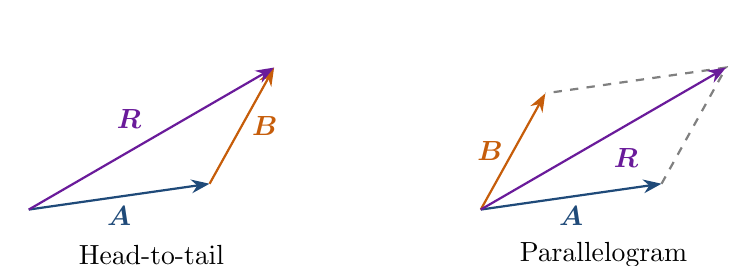
\begin{tikzpicture}[scale=0.82,>=Stealth,thick]
\coordinate (O) at (0,0); \coordinate (A) at (2.8,0.4); \coordinate (B) at (1,1.8); \coordinate (R) at (3.8,2.2);
\draw[->,boxblue] (O)--(A) node[midway,below] {$\vect A$};
\draw[->,boxorange] (A)--(R) node[midway,right] {$\vect B$};
\draw[->,boxpurple] (O)--(R) node[midway,above left] {$\vect R$};
\node at (1.9,-0.7) {Head-to-tail};
\begin{scope}[xshift=7cm]
\draw[->,boxblue] (0,0)--(2.8,0.4) node[midway,below] {$\vect A$};
\draw[->,boxorange] (0,0)--(1,1.8) node[midway,left] {$\vect B$};
\draw[dashed,gray] (2.8,0.4)--(3.8,2.2)--(1,1.8);
\draw[->,boxpurple] (0,0)--(3.8,2.2) node[midway,below right] {$\vect R$};
\node at (1.9,-0.7) {Parallelogram};
\end{scope}
\end{tikzpicture}
\end{center}

\begin{defbox}{Subtract by adding the negative vector}
The vector $-\vect B$ has the same magnitude as $\vect B$ and the opposite direction. Therefore
\[
 \boxed{\vect A-\vect B=\vect A+(-\vect B).}
\]
If $\vect A$ and $\vect B$ share a tail, the arrow \emph{from the head of $\vect B$ to the head of $\vect A$} represents $\vect A-\vect B$. Order matters:
$\vect B-\vect A=-(\vect A-\vect B)$.
\end{defbox}

\begin{rulebox}{Calculate component by component}
\[
 (A_x,A_y)+(B_x,B_y)=(A_x+B_x,A_y+B_y),
\]
\[
 (A_x,A_y)-(B_x,B_y)=(A_x-B_x,A_y-B_y).
\]
In 3D, perform the same operation on the $z$-components. For a real number $c$,
\[
 c\vect A=(cA_x,cA_y,cA_z),\qquad |c\vect A|=|c|\,|\vect A|.
\]
A positive $c$ preserves direction, a negative $c$ reverses it, and $c=0$ produces the zero vector. For $\vect A=(5,3)$, $c\vect A=(5c,3c)$; in particular, $-2\vect A=(-10,-6)$.
\end{rulebox}

\begin{watchbox}
Do not add vector magnitudes unless the directions justify it. In general,
$|\vect A+\vect B|\ne A+B$. For perpendicular vectors,
$|\vect A+\vect B|=\sqrt{A^2+B^2}$; for parallel vectors in the same direction, it is $A+B$; for opposite directions, it is $|A-B|$.
\end{watchbox}

\subsection{Components, Unit Vectors, and Direction Angles}
\bookref{1.8--1.9}{14--19}

\begin{derivbox}{Resolving a vector into components}
Let a nonzero vector $\vect A$ have magnitude $A$ and direction angle $\theta$ measured counterclockwise from $+x$. The horizontal and vertical projections give
\[
 \cos\theta=\frac{A_x}{A},\qquad \sin\theta=\frac{A_y}{A},
 \qquad\boxed{A_x=A\cos\theta,\quad A_y=A\sin\theta.}
\]
These formulas hold in every quadrant when signed sine and cosine values are used. The angle's reference axis is crucial: if the angle is measured from $+y$, the component adjacent to that angle is the $y$-component.
\end{derivbox}

\begin{defbox}{Unit-vector notation}
The Cartesian unit vectors $\uv i$, $\uv j$, and $\uv k$ point along $+x$, $+y$, and $+z$. Each has magnitude one and no physical unit. Write
\[
 \boxed{\vect A=A_x\uv i+A_y\uv j+A_z\uv k.}
\]
For a 2D vector, omit the $z$-term. The coefficients carry the physical units. For any nonzero vector, its own direction unit vector is
\[
 \uv A=\frac{\vect A}{|\vect A|}.
\]
For example, $(3\uv i+4\uv j)/5$ is a unit vector, since its magnitude is one.
\end{defbox}

\begin{rulebox}{Recover magnitude and direction from components}
For a planar resultant,
\[
 R_x=A_x+B_x,\quad R_y=A_y+B_y,\quad
 R=\sqrt{R_x^2+R_y^2}.
\]
If $R_x\ne0$, then $\tan\theta=R_y/R_x$, but an ordinary inverse tangent does not identify the quadrant by itself. First inspect the signs:
\begin{center}
\begin{tabular}{cccc}
\toprule
Quadrant & $R_x$ & $R_y$ & Standard angle\\
\midrule
I & $+$ & $+$ & $0\degree<\theta<90\degree$\\
II & $-$ & $+$ & $90\degree<\theta<180\degree$\\
III & $-$ & $-$ & $180\degree<\theta<270\degree$\\
IV & $+$ & $-$ & $270\degree<\theta<360\degree$\\
\bottomrule
\end{tabular}
\end{center}
Find the acute reference angle $\beta=\tan^{-1}(|R_y/R_x|)$, then choose $\theta=\beta$, $180\degree-\beta$, $180\degree+\beta$, or $360\degree-\beta$, respectively. On an axis, read the direction directly; the zero vector has no direction.
\end{rulebox}

\begin{examplebox}{Compass directions: read the words before choosing sine or cosine}
Take east as $+x$ and north as $+y$.
\begin{itemize}
\item $32\degree$ \textbf{east of north}: start facing north and turn toward east. Then $A_x=A\sin32\degree$, $A_y=A\cos32\degree$. The standard angle is $58\degree$.
\item $36\degree$ \textbf{south of west}: start facing west and turn toward south. Then $B_x=-B\cos36\degree$, $B_y=-B\sin36\degree$. The standard angle is $216\degree$.
\end{itemize}
Both methods agree with $A_x=A\cos\theta$, $A_y=A\sin\theta$ when $\theta$ is the standard angle. A quick sketch fixes the signs before any calculation.
\end{examplebox}

\subsection{Worked Displacement Example: The Buried Keys}
\bookref{1.8, Example 1.7}{18}

\begin{examplebox}{Complete the three-displacement calculation}
The given displacements are
\[
 \begin{aligned}
 \vect A &: 72.4\unit{m},\quad32.0\degree\text{ east of north},\\
 \vect B &: 57.3\unit{m},\quad36.0\degree\text{ south of west},\\
 \vect C &: 17.8\unit{m}\text{ due south}.
 \end{aligned}
\]
\textbf{1. Set up.} Place the origin at the starting point, with east as $+x$ and north as $+y$. We need $\vect R=\vect A+\vect B+\vect C$.

\textbf{2. Resolve each displacement.} Use standard angles $58.0\degree$, $216.0\degree$, and $270.0\degree$:
\begin{align*}
 A_x&=(72.4\unit{m})\cos58.0\degree\approx38.366\unit{m},\\
 A_y&=(72.4\unit{m})\sin58.0\degree\approx61.399\unit{m},\\
 B_x&=-(57.3\unit{m})\cos36.0\degree\approx-46.357\unit{m},\\
 B_y&=-(57.3\unit{m})\sin36.0\degree\approx-33.680\unit{m},\\
 C_x&=0\unit{m},\qquad C_y=-17.8\unit{m}.
\end{align*}
\textbf{3. Add components, keeping unrounded values.}
\[
 R_x\approx-7.99\unit{m},\qquad R_y\approx9.92\unit{m},
 \qquad\boxed{\vect R\approx(-7.99\uv i+9.92\uv j)\unit{m}.}
\]
The signs mean the keys are west and north of the starting point.

\textbf{4. Find the direct distance.}
\[
 R=\sqrt{R_x^2+R_y^2}\approx\boxed{12.7\unit{m}}.
\]
\textbf{5. Find the direction.} The direction is in quadrant II. With
$\beta=\tan^{-1}(|R_y/R_x|)\approx51.1\degree$,
\[
 \theta=180\degree-\beta\approx128.9\degree.
\]
Equivalently, the direction is $\theta-90\degree\approx38.9\degree$ west of north. Report the direct route as
\[
 \boxed{12.7\unit{m},\quad39\degree\text{ west of north}.}
\]
\textbf{6. Check.} The east--west and north--south components nearly cancel, so a short resultant is sensible. The full three-leg route is $72.4+57.3+17.8=147.5\unit{m}$, much longer than the direct displacement's magnitude.
\end{examplebox}

\begin{watchbox}
The value $\tan^{-1}(R_y/R_x)\approx-51.1\degree$ lies in quadrant IV, while the components clearly place the resultant in quadrant II. These angles differ by $180\degree$. Always check the component signs; the calculator cannot infer the intended quadrant from a single ratio.
\end{watchbox}

\subsection{The Scalar or Dot Product}
\bookref{1.10}{20--22}

\begin{defbox}{A vector product whose result is a scalar}
For nonzero vectors $\vect A$ and $\vect B$ separated by angle $0\degree\leq\phi\leq180\degree$,
\[
 \boxed{\vect A\cdot\vect B=AB\cos\phi.}
\]
It measures how strongly the vectors align. The dot product is a scalar; its units are the product of the units of the two vectors. It may be positive, zero, or negative:
\begin{center}
\begin{tabular}{lll}
\toprule
Angle & Dot product & Interpretation\\
\midrule
$0\degree$ & $AB$ & same direction\\
$0\degree<\phi<90\degree$ & positive & acute angle\\
$90\degree$ & $0$ & perpendicular\\
$90\degree<\phi<180\degree$ & negative & obtuse angle\\
$180\degree$ & $-AB$ & opposite directions\\
\bottomrule
\end{tabular}
\end{center}
If either vector is zero, the dot product is zero although the angle is undefined. The converse ``zero dot product implies perpendicular'' therefore assumes both vectors are nonzero.
\end{defbox}

\begin{derivbox}{The component formula}
In perpendicular Cartesian axes,
\[
 \uv i\cdot\uv i=\uv j\cdot\uv j=\uv k\cdot\uv k=1,
 \qquad\uv i\cdot\uv j=\uv j\cdot\uv k=\uv k\cdot\uv i=0.
\]
Expand $(A_x\uv i+A_y\uv j+A_z\uv k)\cdot(B_x\uv i+B_y\uv j+B_z\uv k)$. All cross-axis terms vanish, leaving
\[
 \boxed{\vect A\cdot\vect B=A_xB_x+A_yB_y+A_zB_z.}
\]
For 2D vectors, omit the $z$-term. The dot product is commutative and distributive:
\[
 \vect A\cdot\vect B=\vect B\cdot\vect A,\qquad
 \vect A\cdot(\vect B+\vect C)=\vect A\cdot\vect B+\vect A\cdot\vect C.
\]
Also, $\vect A\cdot\vect A=A^2$, which is a useful magnitude check.
\end{derivbox}

\begin{examplebox}{The component example from the lecture}
\[
 (3,5)\cdot(4,8)=3\times4+5\times8=12+40=\boxed{52}.
\]
The answer is a single number, not $(12,40)$. The vectors were given without physical units; if each had units of metres, the dot product would have units $\mathrm{m^2}$.
\end{examplebox}

\begin{plotbox}{1.27}{Two routes to the same dot product}
\begin{center}
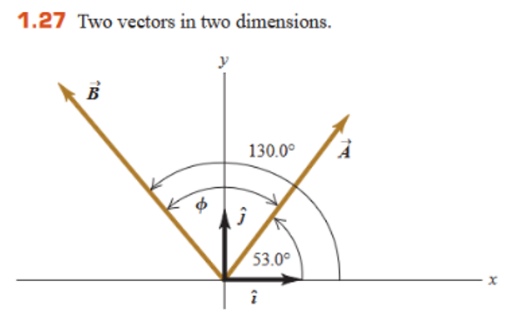
\includegraphics[width=0.66\linewidth]{fig1.27.png}
\end{center}
{\footnotesize Source: Young and Freedman, 13th ed., Fig.\ 1.27, p.\ 22; supplied figure image.}

\medskip
\textbf{Read the angles.} Vector $\vect A$ has magnitude $4.00$ and direction $53.0\degree$ from $+x$; $\vect B$ has magnitude $5.00$ and direction $130.0\degree$. The angle \emph{between} them is
\[
 \phi=130.0\degree-53.0\degree=77.0\degree.
\]
\textbf{Geometric calculation:}
\[
 \vect A\cdot\vect B=(4.00)(5.00)\cos77.0\degree
 =4.4990\ldots\approx\boxed{4.50}.
\]
\textbf{Component check:}
\[
 \begin{aligned}
 \vect A&=(4\cos53\degree,4\sin53\degree)\approx(2.4073,3.1945),\\
 \vect B&=(5\cos130\degree,5\sin130\degree)\approx(-3.2139,3.8302).
 \end{aligned}
\]
Then $A_xB_x+A_yB_y\approx4.50$, as required. The horizontal contribution is negative and the vertical contribution positive; their sum is positive because $77\degree$ is acute. The two individual direction angles are not themselves the angle to insert into $AB\cos\phi$.
\end{plotbox}

\begin{examplebox}{Find the angle between two 3D vectors}
The lecture gives
\[
 \vect A=2\uv i+3\uv j+\uv k,\qquad
 \vect B=-4\uv i+2\uv j-\uv k.
\]
First compute the scalar product and magnitudes:
\[
 \vect A\cdot\vect B=2(-4)+3(2)+1(-1)=-3,
 \quad A=\sqrt{14},\quad B=\sqrt{21}.
\]
Solve the geometric definition for the angle:
\[
 \boxed{\phi=\cos^{-1}\!\left(\frac{\vect A\cdot\vect B}{AB}\right)}
 =\cos^{-1}\!\left(\frac{-3}{\sqrt{14}\sqrt{21}}\right)
 \approx\boxed{100.1\degree}.
\]
A negative dot product requires an obtuse angle, which checks the result. This formula requires two nonzero vectors.
\end{examplebox}

\begin{examplebox}{Physical interpretation: work and projections}
For a constant force and displacement,
\[
 \boxed{W=\vect F\cdot\vect d=Fd\cos\phi.}
\]
Only the component of force along the displacement contributes to the work done by that force. If $F=10\unit{N}$, $d=3\unit{m}$, and $\phi=60\degree$, then $W=15\unit{J}$. A perpendicular force does zero work; a force component opposite to the displacement does negative work.

For a direction unit vector $\uv n$, the signed scalar component of $\vect A$ along that direction is $\vect A\cdot\uv n$. In particular, $A_x=\vect A\cdot\uv i=A\cos\theta$.
\end{examplebox}

\subsection{The Vector or Cross Product}
\bookref{1.10}{23--25}

\begin{defbox}{A vector perpendicular to the input vectors}
In three-dimensional space, define $\vect C=\vect A\times\vect B$. For nonzero input vectors, its magnitude is
\[
 \boxed{|\vect C|=AB\sin\phi,\qquad0\degree\leq\phi\leq180\degree.}
\]
If the inputs are not parallel, $\vect C$ is perpendicular to both, with direction chosen by the right-hand rule. If the inputs are parallel, antiparallel, or one is zero, the cross product is the zero vector and has no direction.

Its magnitude is the area of the parallelogram spanned by the two vectors: base $A$ times perpendicular height $B\sin\phi$. When the input vectors are lengths, this area has units $\mathrm{m^2}$. In general, the cross product's units are the product of the input units.
\end{defbox}

\begin{plotbox}{1.29}{The right-hand rule and reversal of order}
\begin{center}
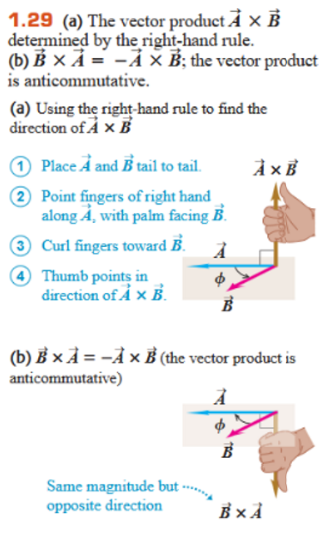
\includegraphics[height=0.40\textheight,keepaspectratio]{fig1.29.png}
\end{center}
{\footnotesize Source: Young and Freedman, 13th ed., Fig.\ 1.29, p.\ 23; supplied figure image.}

\medskip
\textbf{Panel (a).} Place the vectors tail to tail. Point your right-hand fingers along $\vect A$, then curl them toward $\vect B$ through the smaller angle. Your thumb gives the direction of $\vect A\times\vect B$, perpendicular to the plane of the two vectors.

\textbf{Panel (b).} Reversing the order reverses the direction but leaves the magnitude unchanged:
\[
 \boxed{\vect B\times\vect A=-(\vect A\times\vect B).}
\]
The operation is therefore \emph{anticommutative}. It is not enough to find $AB\sin\phi$: a complete nonzero cross product also needs a direction or signed components.
\end{plotbox}

\begin{rulebox}{Unit-vector products in a right-handed system}
The forward cyclic order is $\uv i\to\uv j\to\uv k\to\uv i$:
\[
 \uv i\times\uv j=\uv k,\qquad
 \uv j\times\uv k=\uv i,\qquad
 \uv k\times\uv i=\uv j.
\]
Reversing a product introduces a minus sign. A vector crossed with itself gives zero:
\[
 \uv j\times\uv i=-\uv k,\qquad
 \uv i\times\uv i=\uv j\times\uv j=\uv k\times\uv k=\vect0.
\]
For example, if $\vect A=3\uv i$ and $\vect B=4\uv j$, then
$\vect A\times\vect B=12\uv k$, while $\vect B\times\vect A=-12\uv k$.
\end{rulebox}

\begin{derivbox}{Component formula and determinant mnemonic}
In a right-handed orthonormal Cartesian basis, a convenient arrangement is
\[
 \vect A\times\vect B=
 \begin{vmatrix}
 \uv i&\uv j&\uv k\\
 A_x&A_y&A_z\\
 B_x&B_y&B_z
 \end{vmatrix}.
\]
Expand along the first row, using signs $+,-,+$:
\begin{align*}
 \vect A\times\vect B
 &=(A_yB_z-A_zB_y)\uv i\\
 &\quad-(A_xB_z-A_zB_x)\uv j\\
 &\quad+(A_xB_y-A_yB_x)\uv k.
\end{align*}
Equivalently, the three components are
\[
 \boxed{C_x=A_yB_z-A_zB_y,\quad
 C_y=A_zB_x-A_xB_z,\quad C_z=A_xB_y-A_yB_x.}
\]
The minus sign in front of the $\uv j$ term is already incorporated into the displayed formula for $C_y$; do not apply it twice. You can use these component formulas without knowing general determinant theory.
\end{derivbox}

\begin{rulebox}{Useful checks and planar vectors}
For $\vect C=\vect A\times\vect B$,
\[
 \vect A\cdot\vect C=0,\qquad\vect B\cdot\vect C=0,
 \qquad |\vect C|\leq AB.
\]
If both input vectors lie in the $xy$-plane, append zero $z$-components:
\[
 (A_x,A_y,0)\times(B_x,B_y,0)=(0,0,A_xB_y-A_yB_x).
\]
With $+x$ right and $+y$ up on a page, positive $z$ points out of the page ($\odot$), while negative $z$ points into it ($\otimes$). The cross product is perpendicular to the page, not another arrow within it.
\end{rulebox}

\begin{watchbox}
The dot product uses \textbf{cosine} and produces a \textbf{scalar}; the magnitude of the cross product uses \textbf{sine} and the cross product produces a \textbf{vector}. For nonzero parallel vectors the cross product vanishes; for perpendicular vectors the dot product vanishes. Do not swap these statements.
\end{watchbox}

\newpage
\subsection*{Quick Reference and Common Exam Traps}
\addcontentsline{toc}{subsection}{Quick Reference and Common Exam Traps}
\begin{rulebox}{Core formula sheet}
\begin{align*}
 \text{Speed and density:}\quad &v_{\rm av}=d/\Delta t,\qquad\rho=m/V,\\
 \text{Planar components:}\quad&A_x=A\cos\theta,\qquad A_y=A\sin\theta,\\
 \text{Magnitude:}\quad&A=\sqrt{A_x^2+A_y^2+A_z^2},\\
 \text{Sum components:}\quad&R_i=A_i+B_i,\\
 \text{Dot product:}\quad&\vect A\cdot\vect B=AB\cos\phi\\
 &\hspace{2.8em}=A_xB_x+A_yB_y+A_zB_z,\\
 \text{Angle between vectors:}\quad&\cos\phi=\frac{\vect A\cdot\vect B}{AB},\\
 \text{Cross-product magnitude:}\quad&|\vect A\times\vect B|=AB\sin\phi.
\end{align*}
Here $i$ in $R_i=A_i+B_i$ means any coordinate $x,y,z$; it is not the unit vector $\uv i$. The angle formula requires nonzero vectors.
\[
 1\unit{N}=1\unit{kg\,m\,s^{-2}},\quad
 1\unit{J}=1\unit{N\,m},\quad1\unit{Pa}=1\unit{N\,m^{-2}},
\]
\[
 1\unit{N}=10^5\unit{dyne},\quad
 1\unit{J}=10^7\unit{erg},\quad
 1\unit{g\,cm^{-3}}=10^3\unit{kg\,m^{-3}}.
\]
\end{rulebox}

\begin{center}
\begin{tabular}{lll}
\toprule
\textbf{Feature} & \textbf{Dot product} & \textbf{Cross product}\\
\midrule
Result & scalar & vector\\
Geometric formula & $AB\cos\phi$ & magnitude $AB\sin\phi$\\
Swap the inputs & unchanged & sign reversed\\
Parallel nonzero inputs & $+AB$ or $-AB$ & zero vector\\
Perpendicular inputs & zero & magnitude $AB$\\
Physical application & work & torque\\
\bottomrule
\end{tabular}
\end{center}

\begin{watchbox}
Before accepting an answer, check these five things:
\begin{enumerate}
\item \textbf{Units:} have you converted grams to kilograms and squared or cubed the length conversion where needed?
\item \textbf{Angle convention:} is the given angle measured from $+x$, from north, or between two vectors?
\item \textbf{Signs and quadrant:} does the answer point in the direction indicated by the components?
\item \textbf{Type of answer:} should the result be a scalar, a vector, or a vector's magnitude?
\item \textbf{Size:} a resultant satisfies $|A-B|\leq|\vect A+\vect B|\leq A+B$, while $|\vect A\cdot\vect B|\leq AB$ and $|\vect A\times\vect B|\leq AB$.
\end{enumerate}
\end{watchbox}

\newpage
\subsection*{Practice Problems}
\addcontentsline{toc}{subsection}{Practice Problems}

\subsubsection*{A. Multiple-choice questions}
Choose one answer in each case.

\begin{enumerate}[label=\textbf{\arabic*.}]
\item A sample has density $1.2\unit{g\,cm^{-3}}$. In SI units this is:\\
\textbf{A} $1.2\unit{kg\,m^{-3}}$; \textbf{B} $12\unit{kg\,m^{-3}}$; \textbf{C} $120\unit{kg\,m^{-3}}$; \textbf{D} $1200\unit{kg\,m^{-3}}$; \textbf{E} $12000\unit{kg\,m^{-3}}$.
\item Which expression is equivalent to one joule?\\
\textbf{A} $\mathrm{kg\,m\,s^{-1}}$; \textbf{B} $\mathrm{kg\,m^2\,s^{-2}}$; \textbf{C} $\mathrm{kg\,m^{-1}\,s^{-2}}$; \textbf{D} $\mathrm{kg\,m\,s^{-2}}$; \textbf{E} $\mathrm{kg\,m^2\,s^{-1}}$.
\item A displacement is $10\unit{m}$, $30\degree$ east of north. Its eastward component is:\\
\textbf{A} $5\unit{m}$; \textbf{B} $5\sqrt3\unit{m}$; \textbf{C} $10\unit{m}$; \textbf{D} $-5\unit{m}$; \textbf{E} $0\unit{m}$.
\item Two nonzero vectors are perpendicular. Which statement must hold?\\
\textbf{A} Their sum is zero; \textbf{B} their magnitudes are equal; \textbf{C} their cross product is zero; \textbf{D} their dot product is negative; \textbf{E} their dot product is zero.
\item For $\vect A=2\uv i$ and $\vect B=3\uv j$, what is $\vect B\times\vect A$?\\
\textbf{A} $6\uv k$; \textbf{B} $-6$; \textbf{C} $-6\uv k$; \textbf{D} $\vect0$; \textbf{E} $6\uv i$.
\item A vector has components $(-3,4)$. Its magnitude and quadrant are:\\
\textbf{A} $7$, II; \textbf{B} $5$, II; \textbf{C} $5$, IV; \textbf{D} $-5$, II; \textbf{E} $1$, I.
\item Convert $2.0\unit{cm^3}$ to $\mathrm{m^3}$.\\
\textbf{A} $2.0\times10^{-2}$; \textbf{B} $2.0\times10^{-3}$; \textbf{C} $2.0\times10^{-4}$; \textbf{D} $2.0\times10^{-6}$; \textbf{E} $2.0\times10^6$.
\item Vectors have magnitudes 3 and 4. Which cannot be the magnitude of their sum?\\
\textbf{A} $0$; \textbf{B} $1$; \textbf{C} $3$; \textbf{D} $5$; \textbf{E} $7$.
\end{enumerate}

\subsubsection*{B. Exercise 1.12: Vector operations}
The vectors below are given without physical units. Use equal scales on the coordinate axes. In part (c), measure the angle from the positive $x$-axis in three dimensions. The labels $\vect c_{\rm sum}$ and $\vect c_{\rm cross}$ distinguish the results of parts (c) and (d).

\begin{enumerate}[label=\textbf{(\alph*)}]
\item Draw $\vect u=(2.5,1.0)$ and $\vect v=(-0.5,-2.0)$. Plot $\vect v+\vect u$ and $\vect u-\vect v$. Calculate $\vect u\cdot\vect v$.
\item For $\vect a=(2,-4,1)$ and $\vect b=(4,5,2)$, calculate $\vect a\cdot\vect b$.
\item Calculate $\vect c_{\rm sum}=\vect a+\vect b$, its length, and its angle $\theta$ to the positive $x$-axis.
\item Calculate $\vect c_{\rm cross}=\vect a\times\vect b$ and its length. Verify that your result is perpendicular to both inputs.
\end{enumerate}

\subsubsection*{C. Displacement problems}
\begin{enumerate}[label=\textbf{\arabic*.},start=9,itemsep=1.1em]
\item \textbf{Fence posts.} A fence post is $52.0\unit{m}$ from where you are standing, in a direction $37.0\degree$ north of east. A second fence post is due south of you. What is the distance of the second post from you if the distance between the two posts is $80.0\unit{m}$?

\item \textbf{A dog in an open field (Young--Freedman, Problem 1.83).} A dog runs $12.0\unit{m}$ east and then $28.0\unit{m}$ in a direction $50.0\degree$ west of north. In what direction and how far must the dog then run to end up $10.0\unit{m}$ south of her original starting point?

\item \textbf{A sailboat in shifting winds (Young--Freedman, Problem 1.72).} A sailor sails $2.00\unit{km}$ east, then $3.50\unit{km}$ southeast, and then an additional distance in an unknown direction. Her final position is $5.80\unit{km}$ directly east of the starting point. Find the magnitude and direction of the third leg of the journey. Draw the vector-addition diagram and show that it is in qualitative agreement with your numerical solution.
\end{enumerate}

\end{document}
